\section{引言}
\label{sec:introduction}

机器人操作策略在静态场景中已取得显著进展 \cite{diffusionpolicy,pi05}。在这类场景中，世界在推理期间保持静止，动作执行时仍可依据先前的观测。
在动态操作中，目标在推理期间持续运动，观测到的位姿在动作执行时已经过时。例如，物块以约 0.9\,m/s 的速度沿斜坡滑动，在 200\,ms 的推理期间会移动 18\,cm，远超精确接触允许的位置误差。
成功操作因此需要预测目标在动作执行时的位姿。策略还必须考虑可能阻挡接近路径或改变目标运动的周围物体。预测本身也需要时间。更耗时的预测会推迟动作执行，并延长策略必须预测的时间跨度。这使预测精度与及时行动之间产生矛盾。

现有方法预测的内容各有不同（图~\ref{fig:paradigms}）。场景级方法预测未来图像或视频 \cite{dbctfp,dreamzero,openwam_alpha,dynamicwam}，或预测 3D 运动 \cite{physmani}。这些预测能覆盖周围环境的运动，但稠密预测可能把计算花在与接触关系不大的区域。视频预测中，目标可能只占画面的一小部分，其位姿仍隐含在预测的像素中。
AHEAD 只对任务相关的隐空间图像块做预测 \cite{ahead}，PUMA 用目标的未来特征做监督 \cite{domino}，SPOT 预测目标的位姿轨迹 \cite{spot}。聚焦目标可能遗漏阻挡接近路径或改变目标运动的周围物体。例如，即使目标沿预测轨迹运动，移动障碍物仍可能阻断接近路径。判断路径是否畅通与估计接触时的目标位姿，对预测有不同要求。
我们的问题是，\emph{为了及时准确地完成接触，需要预测运动场景中的什么，又需要多高的精度？}

\begin{figure}[t]
\centering
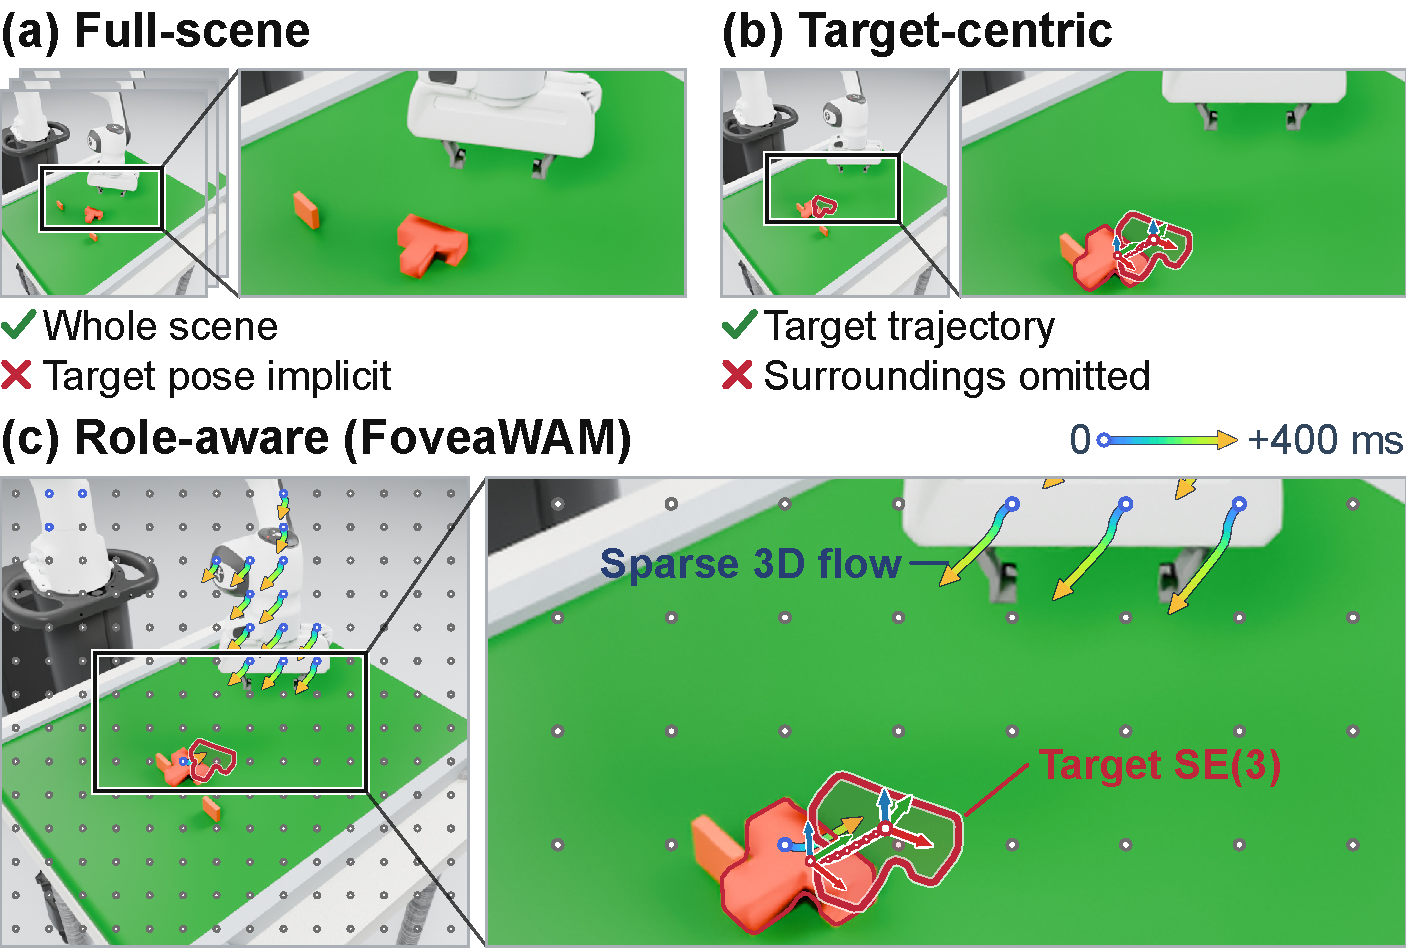
\includegraphics[width=\columnwidth]{figures/paradigms/paradigms.pdf}
\caption{\textbf{预测精度如何分配。}
(a) 全场景方法（如视频世界—动作模型）预测整个场景的未来帧，目标位姿隐含其中 \cite{dreamzero,openwam_alpha}。
(b) 以目标为中心的方法只预测目标的运动，省略周围环境 \cite{domino,spot}。
(c) \ours 为目标预测精确的 SE(3) 轨迹，为周围环境只预测稀疏 3D 流。}
\label{fig:paradigms}
\end{figure}


我们的核心洞见是，\textbf{预测需求因角色而异}（图~\ref{fig:teaser}）。目标在动作执行时的位置和朝向直接决定接触是否成功，需要精确预测。
周围物体通过阻挡接近路径或改变目标运动间接影响接触，粗略预测它们的运动即可。其余场景是静态的，可直接从当前帧获得，无需预测。
策略因此可以集中精确预测目标，并以较低代价刻画周围环境，及时完成准确接触。生物视觉也有类似分工，中央凹分辨细节，周边视野感知大范围的运动 \cite{curcio1990photoreceptor,strasburger2011peripheral,rosenholtz2016peripheral}。

我们据此提出 \textbf{\ours}，一个按角色分配精度的原生 4D 世界—动作模型（图~\ref{fig:paradigms}c）。\ours 直接在度量 3D 空间中随时间观测和预测场景运动，而非在像素空间中。在这一空间中，场景各部分可以分别表示，并获得其角色所需的精度。
模型用一条度量 SE(3) 轨迹精确预测目标，仅用少量参数显式给出其未来位置和朝向，用稀疏 3D 流粗略预测周围物体的运动，对静态场景不做预测。
同样的分配也适用于输入。单帧可提供静态环境与周围物体的布局，只有目标的运动需要历史。
\ours 因此输入一帧 RGB-D 和一段短的目标 SE(3) 位姿历史。现有动态策略使用历史图像或光流~\cite{dynamicvla,domino,dynamicwam}。
紧凑的输入与预测使 \ours 在单张 \cfgGPU{} 上 15.1\,ms 内给出动作，速度约为视频世界—动作模型的 10 倍，缩短了动作执行前场景继续运动的时间。

评估预测精度与行动时机的权衡需要计入推理时间。DOMINO \cite{domino} 和 PhysMani-Bench \cite{physmani} 默认在推理期间暂停仿真，相当于把慢策略也视为即时执行。
为此，我们提出包含 14 个动态操作任务的基准 \textbf{\bench}。仿真在推理期间持续运行，每个策略都按原生延迟接受评测。在同一组场景上，暂停仿真会高估慢策略的表现，并改变方法的排名（图~\ref{fig:latency}c）。

实验表明，\ours 能及时完成准确接触。在 \bench 上，其原生延迟下的成功率为 82.1\%，比最强基线高 \nativeLead{} 个百分点。
在 DOMINO \cite{domino} 的单臂任务上，\ours 同样领先 19.9 个百分点。其评测器在推理期间暂停仿真，因此这一优势并非仅来自速度。
在六项真机任务上，\ours 在每项任务中均取得最高成功率，平均为 48.3\%，比最强基线高 17.5 个百分点。
消融实验显示，角色感知设计的各部分均有贡献，其中移除目标位姿历史造成的成功率下降最大。

我们的贡献有三点：
\begin{itemize}[leftmargin=*,topsep=2pt,itemsep=1pt]
\item 我们明确了动态操作中目标、周围物体和静态场景各自的预测需求，并提出按角色分配精度的预测范式。它精确预测目标运动，粗略预测周围物体的运动，并用当前帧获取静态几何，在保留接触所需精度的同时降低计算开销。
\item 我们提出 \textbf{\ours}，一个实现这一范式的原生 4D 世界—动作模型，可精确、低延迟地生成动作。它在 15.1\,ms 内给出动作，速度约为视频世界—动作模型的 10 倍，在 \bench 上领先最强基线 \nativeLead{} 个百分点，在推理期间暂停仿真的 DOMINO 单臂任务以及六项动态真机任务上也取得领先。
\item 我们提出 \textbf{\bench}，一个包含 14 个动态操作任务的基准，其中世界从不暂停，每个策略都在其原生延迟下接受评测，从而揭示了暂停式评测所掩盖的延迟代价。
\end{itemize}
